\documentclass{beamer}
\usepackage{multirow}
\DeclareMathOperator*{\bb}{\usebeamertemplate***{itemize item}}
\usetheme{default} 
\title{Streamline Curvature Wall Model for Pressure from PIV}
\author{Julian Powers\texorpdfstring{$^1$}{1}, Adrián Lozano-Durán\texorpdfstring{$^2$}{2}}
\institute{
    \tiny
    \texorpdfstring{$^1$}{1}
    Masters Student\\
    Massachusetts Institute of Technology \\[0.5cm]
    \texorpdfstring{$^2$}{1}
    Faculty\\
    Massachusetts Institute of Technology\\ 
    California Institute of Technology\\[0.5cm]
    }
\date{APS DFD, November 2024}



\begin{document}


% Title Slide
\begin{frame}
    \titlepage
\end{frame}


\begin{frame}{Motivation: Why Pressure from PIV?}
    \vspace{0.5cm}
    \begin{table}
        \centering
        \begin{tabular}{p{0.45\textwidth}p{0.45\textwidth}}
            \textbf{Pressure Taps} & \textbf{Pressure from PIV} \\
            \begin{itemize}
                \item Measurements dependent on leakage, hole diameter, flushness
                \item Difficult to install
                \item Length of tubing limits sampling rate
            \end{itemize} & 
            \begin{itemize}
                \item Completely non-invasive
                \item High time resolution possible
                \item High spatial resolution possible
            \end{itemize}\\[-1cm]
            \centering
            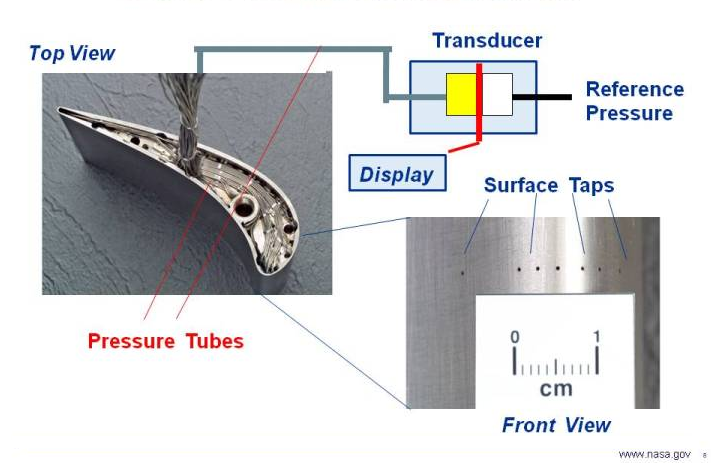
\includegraphics[width=0.5\textwidth]{figs/for_pres/taps.png} & 
            \centering
            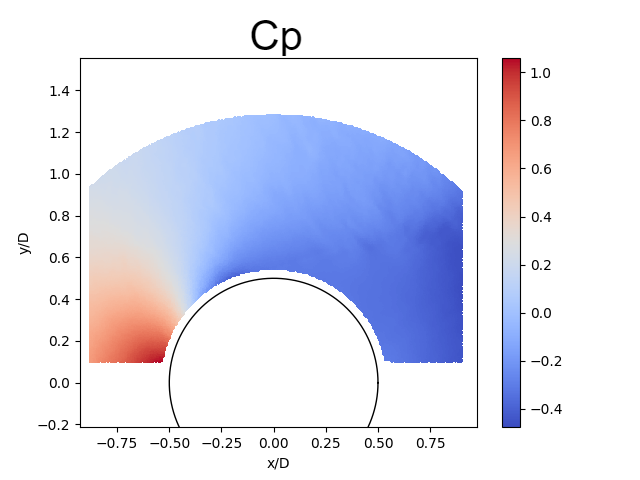
\includegraphics[width=0.5\textwidth]{figs/for_pres/cylinder_full.png}
        \end{tabular}
    \end{table}
\end{frame}


\begin{frame}{Previous Works on Extracting Surface Pressure from PIV}
    \resizebox{\textwidth}{!}{
    \begin{tabular}{|c|c|c|c|}
        \hline
            Case         & Max Cp Error & Extrapolation Approach & Source                 \\
            \hline
            NACA 0012    & 0.5          & parabola fit           & Tagliabue et al., 2017 \\
            Sphere       & 0.15         & nearest neighbor       & Jux et al., 2020       \\
            Cyclist      & 0.2*         & nearest neighbor       & Jux et al., 2020       \\
            Bullet Step  & 0.02         & nearest neighbor       & Gent et al., 2018      \\
            NACA 0012    & 0.25         & line fit               & Ragni et al., 2009     \\
        \hline
    \end{tabular}
    }
    \footnotesize{*based on uncertainty analysis (no pressure tap reference)}
    \begin{tabular}{ccccc}
        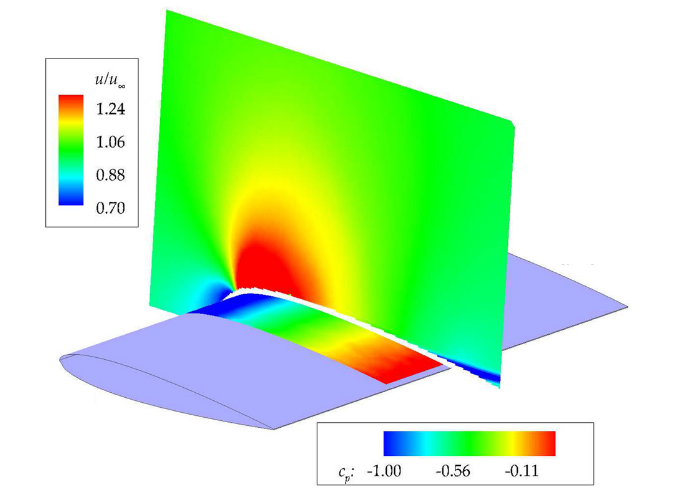
\includegraphics[width = 0.17\textwidth]{figs/for_pres/0012_tagliabue.png} &
        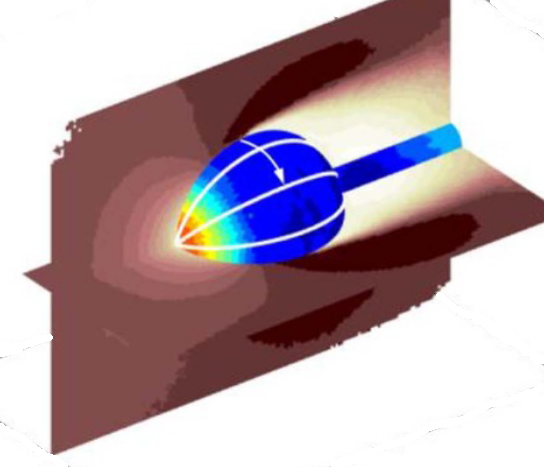
\includegraphics[width = 0.15\textwidth]{figs/for_pres/sphere.png} &
        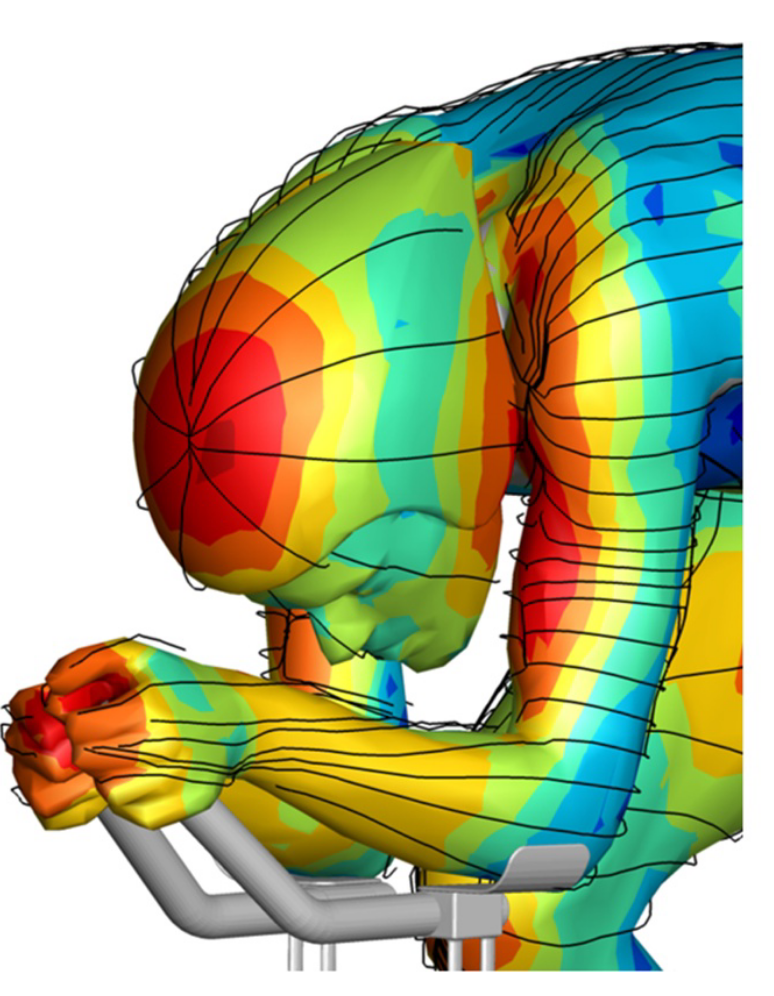
\includegraphics[width = 0.13\textwidth]{figs/for_pres/cyclist.png} &
        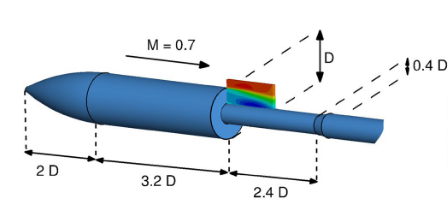
\includegraphics[width = 0.20\textwidth]{figs/for_pres/bullet_step.png} &
        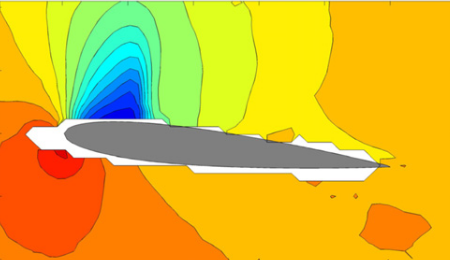
\includegraphics[width = 0.16\textwidth]{figs/for_pres/0012_ragni.png} 
    \end{tabular}
\end{frame}


\begin{frame}{Common Challenges}
    \begin{tabular}{ll}
        $\bb$ Reflections           & \multirow{3}{*}{\Bigg\} degrade near wall velocity data}  \\[2pt]
        $\bb$ Low Particle Density  & \\[2pt]                        
        $\bb$ Turbulence            & \\[2pt]
        $\bb$ Wall Curvature        & \multirow{2}{*}{\Big\} degrade near wall gradient calculations}  \\[2pt]
        $\bb$ Boundary Layers       &                    
    \end{tabular}
    \\[1cm]
    Typical workflow:
    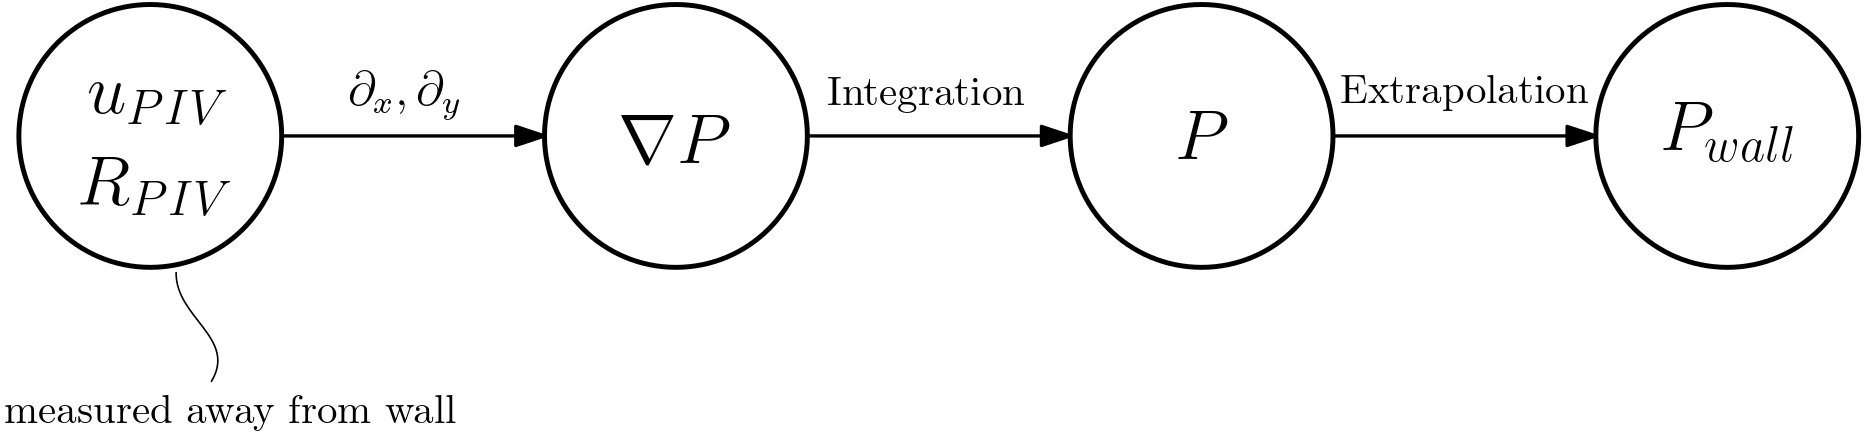
\includegraphics[width=\textwidth]{figs/for_pres/standard_workflow.png}
\end{frame}


\begin{frame}{Idea: Use geometry to calculate $\nabla P$}
\end{frame}


\begin{frame}{Pressure Gradient in Streamline Coordinates}
    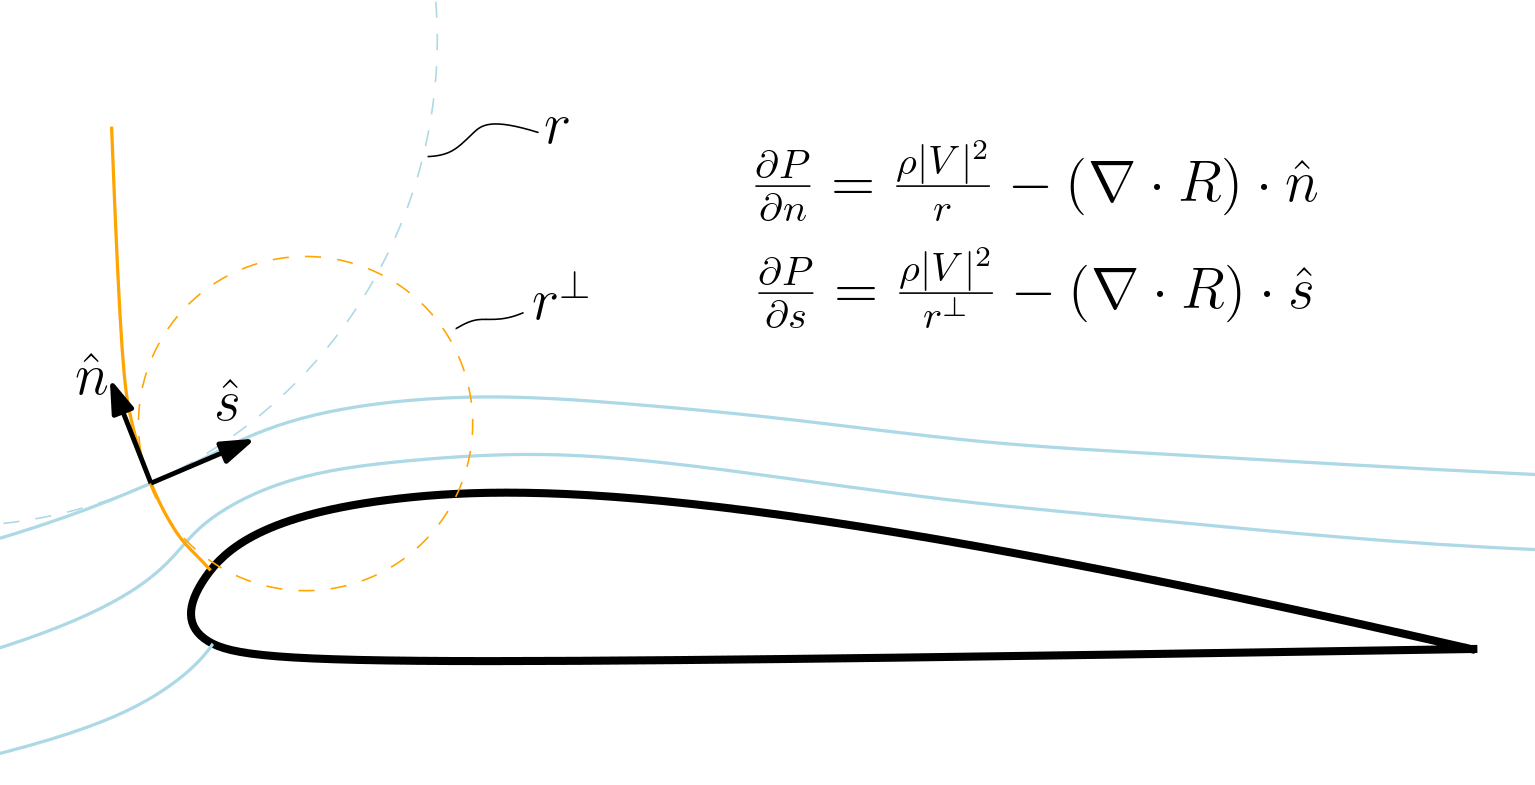
\includegraphics[width=\textwidth]{figs/for_pres/streamlines.png}
\end{frame}


\begin{frame}{Summary of the New Method}
    \begin{enumerate}
        \item Compute Streamlines
        \item Fit Circles
        \item Integration
        \item Differentiation
    \end{enumerate}
\end{frame}


\begin{frame}{LES Airfoil Validation}
    \begin{itemize}
        \item Data from Asada and Kawai, 2018
        \item Grid coarsened from LES
        \item Added 2\% random velocity error
    \end{itemize}
\end{frame}


\begin{frame}{Experimental Setup}
\end{frame}


\begin{frame}{Rough Cylinder Expirimental Results}
\end{frame}


\begin{frame}{Conclusions and Next Steps}
    \begin{itemize}
        \item Robust to noise
        \item Robust to distance from wall
        \item Similar or better results in regions with strong pressure gradient
    \end{itemize}
    \textbf{Next Steps:}
    \begin{itemize}
        \item Improve treatment of Reynolds stresses
        \item Improve treatment of critical points (separation, stagnation point)
        \item Generalization to 3D
    \end{itemize}
\end{frame}



\end{document}
